\documentclass[../book.tex]{subfiles}

\chapter{Diagramming machines}
\label{ch:diagram}

\begin{quote}
Machine learning is not magic; it cannot get something from nothing.
What it does is get more from less. Programming, like all engineering,
is a lot of work: we have to build everything from scratch. Learning is
more like farming, which lets nature do most of the work. Farmers
combine seeds with nutrients to grow crops. Learners combine knowledge
with data to grow programs. \autocite[81]{Domingos_2012}
\index{Domingos, Pedro}
\end{quote}

\begin{quote}
The tools or material machines have to be chosen first of all by a
diagram \autocite[39]{Deleuze_1988} \index{Deleuze, Gilles}
\index{diagram}
\end{quote}

The `learning' in machine learning embodies a change in programming
practice or indeed the programmability of machines. Our sense of the
potentials of machine learning can be understood, according to Pedro
Domingos, in terms of a contrast between programming as `a lot of
{[}building{]} work' and the `farming' done by machine learners to `grow
programs.' In characterising machine learning, the tensions between the
programming `we' (programmers, computer scientists?) do and the
programming that learners do (`growing') are worth pursuing.
\index{programming!human vs. machine} While Domingos suggests that
machine learners `get more from less,' I will propose that an immense
constellation of documents, software, publications, blog pages, books,
spreadsheets, databases, data centre architectures, whiteboard and
blackboard drawings, and an inordinate amount of talk and visual media
orbit around machine learning. \index{programmability!problem of} There
has been lively growth in machine learning, but this liveliness and the
sometimes life-like growth of machine learners are a regional expression
of a distributed formation. `Wherever there is a region of nature,' the
philosopher Alfred North Whitehead writes `which is itself the primary
field of the expressions issuing from each of its parts, that region is
alive' \autocite[31]{Whitehead_1956}.
\index{Whitehead, Alfred North!life}

In this chapter I attend to the problem of identifying and describing
the distributed practices that give rise to a sense of machine learners
framed as growth, or liveliness. I will argue these practices can only
be traced partially through code written in generic or specialized
programming languages such as \texttt{Python} and \texttt{R}, in
libraries of machine learning code such as \texttt{R}'s \texttt{caret}
\index{R!packages!\texttt{caret}} or \texttt{Python}'s
\texttt{scikit-learn} \index{Python!packages!\texttt{scikit-learn}} or
\texttt{TensorFlow} \index{Google!TensorFlow} to do machine learning.
Code obscures and reveals multiple transformations at work in the
operational formation. Science studies scholars such as Anne-Marie Mol
have urged the need to keep practice together with theories of what
exists. Mol writes:

\begin{quote}
If it is not removed from the practices that sustain it, reality is
multiple. This may be read as a description that beautifully fits the
facts. But attending to the multiplicity of reality is also an act. It
is something that may be done -- or left undone \autocite[6]{Mol_2003}
\index{Mol, Anne-Marie}
\end{quote}

Mol advocates thinking reality as multiplicity. Her insistence on the
nexus of practice or doing and the plural existence of things suggests a
way of handling the code that machine learners produce. \index{practice}
Code should be approached multiplicity. In the case of machine learners,
this means following through pedagogical expositions of machine learning
focused on both mathematical derivations and the accumulation of
scientific or technical research publications, ranging from textbooks to
research articles, that vary, explore, experiment and implement machine
learners in code. The effect of liveliness or growth issues from many
parts. In relation to machine learning, reading and writing code
alongside scientific papers, Youtube lectures, machine learning books
and competitions is not only a form of observant participation, but
directly forms part of the diagrammatic multiplicity.

While machine learning utterly depends on code, I will suggest therefore
that no matter how expressive or well-documented it may be, code alone
cannot fully \gls{diagram} how machine learners make programs or how
they combine knowledge with data. Domingos writes that `learning
algorithms \ldots{} are algorithms that make other algorithms. With
machine learning, computers write their own programs, so we don't have
to' \autocite[6]{Domingos_2015a}. Yet the writing performed by machine
learners cannot be read textually or procedurally as other programs
might be read for instance in work known as critical code studies. The
difference between the reading of an Atari computer game console in Nick
Montfort and Ian Bogost's \emph{Racing the Beam}
\autocite{Montfort_2009} and the machine learning of Atari's games
undertaken by DeepMind in London during recent years
\autocites{Mnih_2013}{Mnih_2015} is hard to read from program code.
\index{code!readability of} The learning or making by learning is far
from homogeneous, stable or automatic in practice. Materially, code is
only one element in the diagram of machine learning. It displays, with
greater or lesser degrees of visibility relations between a variety of
forces (infrastructures, scientific knowledges, mathematical
formalisations, etc.). It itself is aligned by and exposes other
institutional, infrastructural, epistemic and economic positions.
\index{code!agency of}

Coding practices and the pedagogical expositions of machine learning
have shifted substantially over the last decade or so due to the growth
in open source programming languages and as a part of the broader and
well-known expansion of digital media cultures. The fact that data
scientists, software developers and other machine learners across
scientific and commercial settings use programming languages such as
\texttt{Python} and \texttt{R}
\index{Python|seealso{programming language}}
\index{R|seealso{programming language!R}} more than specialized
commercial statistical and data software packages such as
\texttt{Matlab}, \texttt{SAS} or \texttt{SPSS} \autocite{Muenchen_2014}
is perhaps symptomatic of shifts in computational culture. Coding
cultures are crucial to the recent growth of machine learning. Although
scientific computing languages such as \texttt{FORTRAN} -- `Formula
Translator' -- have long underpinned scientific research and engineering
applications in various fields
\autocite[34-35]{Campbell-Kelly_2003},\index{programming languages!FORTRAN}
the development in recent decades of data-analytic and statistical
programming languages and coding frameworks has crystallized a
repertoire of standard operations, patterns and functions for reshaping
data and constructing models that classify and predict events and
associations between things, people, processes, etc. This development
continues apace, especially in research and engineering driven by social
media and internet platforms such as Facebook and Google. While Domingos
speaks of `growing' programs, the accumulating sediment of certain
well-established data practices are the soil in which programs take
root. The different elements of coding practice are precisely the
faceted levels of abstraction which we need to access and traverse in
order to know and come to grips empirically with contemporary
compositions of power and knowledge in machine learning.
\index{code!writing of}

\section{\texorpdfstring{`We don't have to write
programs'?}{We don't have to write programs?}}\label{we-dont-have-to-write-programs}

In machine learning, coding changes from what we might call symbolic
logical diagrams to statistical algorithmic diagrams. While many machine
learning techniques have long statistical lineages (running back to the
1900s in the case of Karl Pearson's development of the still-heavily
used Principal Component Analysis \autocite{Pearson_1901}),
\index{Pearson, Karl}\index{machine learner!principal component analysis}
machine learning techniques often embody a certain dissatisfaction with
the classical computer science understanding of programs as manipulation
of symbols, even as they rely on such symbolic operations to function.
Symbolic manipulation, epitomised by deductive logic or predicate
calculus, was very much at the centre of many AI projects during the
1950s and 1960s \autocites{Dreyfus_1972}{Edwards_1996}.
\index{artificial intelligence!symbolic manipulation in} In machine
learning, the privileged symbolic-cognitive forms of logic are subject
to a statistical transformation.

Take for instance once of the most common operations of the Boolean
logical calculus, the \texttt{NOT-AND} or \texttt{NAND} function shown
in table \ref{tab:boolean}. The truth table summarises a logical
function \index{function!logical} that combines three input variables
\texttt{X1}, \texttt{X2}, and \texttt{X3} and produces the output
variable \texttt{Y}. Because in Boolean calculus, variables or
predicates can only take the values \texttt{true} or \texttt{false},
they can be coded in as \texttt{1} and \texttt{0}.

\begin{longtable}[c]{@{}llll@{}}
\caption{The truth table for the Boolean function NOT-AND truth
\label{tab:boolean}}\tabularnewline
\toprule
X1 & X2 & X3 & Y\tabularnewline
\midrule
\endfirsthead
\toprule
X1 & X2 & X3 & Y\tabularnewline
\midrule
\endhead
0 & 0 & 0 & 1\tabularnewline
0 & 0 & 1 & 1\tabularnewline
0 & 1 & 1 & 1\tabularnewline
0 & 1 & 0 & 1\tabularnewline
1 & 0 & 0 & 1\tabularnewline
1 & 0 & 1 & 1\tabularnewline
1 & 1 & 0 & 1\tabularnewline
1 & 1 & 1 & 0\tabularnewline
\bottomrule
\end{longtable}

Now in Foucaultean terms, the truth table and its component propositions
constitutes a statement. This statement has triple relevance for
\gls{archaeology} of machine learning.
\index{statements!truth tables as} The spatial arrangement of the table
is fundamental (and this is the topic of chapter \ref{ch:vector}).
\index{table!see {data!table}} Most datasets come as tables, or end up
as tables at some point in their analysis. Second, the elements or cells
of this table are numbers. The numbers \(1\) and \(0\) are the binary
digits as well as the `truth' values `True' and `False' in classical
logic. These numbers are readable as symbolic logical propositions
governed by the rule \(Y = \neg{X_1 \land X_2 \land X_3}\). The table
acts as a hinge between numbers and symbolic thought or cognition.
Third, the NAND table in particular has an obvious operational relevance
in digital logic, since digital circuits of all kinds -- memory,
processing, and communication -- comprise such logical functions knitted
together in the intricate gated labyrinths of contemporary
calculation.\footnote{The philosophy Charles Sanders Peirce himself
  \index{Peirce, Charles Sanders!on NAND operation} had first shown that
  combinations of NAND operations could stand in for any logical
  expression whatsoever, thus paving the way for the diagrammatic weave
  of contemporary digital memory and computation in all their
  permutations. Today, NAND-based logic is norm in digital electronics.
  NOR -- NOT OR -- logic is also used in certain applications.}
\index{infrastructure!digital circuit as}

A pre-machine learning programmer, tasked with implementing the logical
NAND function might write:

\begin{lstlisting}[language=Python, caption={XOR function in Python}, label={lst:nand}]
Y = not(X1 & X2 & X3)
\end{lstlisting}

The trivial simplicity of the code stands out. This looks like the kind
of symbol manipulation that that computers can easily be programmed to
do. How, by contrast, could such a truth table be learned by a machine,
even a machine whose \emph{modus operandi} and indeed whose very fabric
is nothing other than a massive mosaic of \texttt{NAND} operations
inscribed in semiconductors? Machine learning of on elementary truth
tables is not a typical operation today, but usefully illustrates
something of the diagrammatic transformations that programming or coding
(and classical AI) has undergone \index{artificial intelligence}.

Machine learners such as decision trees or neural nets typically know
nothing of the logical calculus and its elementary logical operations.
Can they be induced to learn it? A perceptron, an elementary machine
learner dating from the
1950s,\index{machine learner!perceptron!learning logical functions} that
`learns' the binary logical operation NAND (Not-AND) is expressed in
twenty lines of python code on the Wikipedia `Perceptron' page
\autocite{Wikipedia_2013} (see listing \ref{lst:perceptron_code}). It is
a standard machine learner almost always included in machine learning
textbooks and usually taught in introductory machine learning classes.
The code outputs a series of numbers shown in table
\ref{tab:nand_weights}.

\begin{lstlisting}[language=Python, caption={Perceptron learning $XOR$ function}, label={lst:perceptron_code}]

threshold = 0.5
learning_rate = 0.1
weights = [0, 0, 0]
training_set = [((1, 0, 0), 1), ((1, 0, 1), 1), ((1, 1, 0), 1), ((1, 1, 1), 0)]

def dot_product(values):
    return sum(value * weight for value, weight in zip(values, weights))

out = 'weight1, weight2, weight3, error_count, iteration'
print  out
iteration_count = 0
while True:
    error_count = 0
    iteration_count += 1
    for input_vector, desired_output in training_set:
        out = ','.join(map(str,weights)) + ',' + str(error_count)
        out = out + ',' + str(iteration_count)
        result = dot_product(input_vector) > threshold
        error = desired_output - result
        print out
        if error != 0:
            error_count += 1
            for index, value in enumerate(input_vector):
                weights[index] += learning_rate * error * value
    if error_count == 0:
        break
\end{lstlisting}

\begin{table}[!htb]
\centering
\begingroup\tiny
\begin{tabular}{rrrrr}
  \hline
weight1 & weight2 & weight3 & error\_count & iteration \\ 
  \hline
0.00 & 0.00 & 0.00 &   0 &   1 \\ 
  0.10 & 0.00 & 0.00 &   1 &   1 \\ 
  0.20 & 0.00 & 0.10 &   2 &   1 \\ 
  0.30 & 0.10 & 0.10 &   3 &   1 \\ 
  0.30 & 0.10 & 0.10 &   0 &   2 \\ 
  0.40 & 0.10 & 0.10 &   1 &   2 \\ 
  0.50 & 0.10 & 0.20 &   2 &   2 \\ 
  0.50 & 0.10 & 0.20 &   2 &   2 \\ 
  0.40 & 0.00 & 0.10 &   0 &   3 \\ 
  0.50 & 0.00 & 0.10 &   1 &   3 \\ 
  0.50 & 0.00 & 0.10 &   1 &   3 \\ 
  0.60 & 0.10 & 0.10 &   2 &   3 \\ 
  0.50 & 0.00 & 0.00 &   0 &   4 \\ 
  0.60 & 0.00 & 0.00 &   1 &   4 \\ 
  0.60 & 0.00 & 0.00 &   1 &   4 \\ 
   \hline
\end{tabular}
\endgroup
\caption{Iterative change in weights as a perceptron learns the NAND function} 
\label{tab:nand_weights}
\end{table}

What does the code in listing \ref{lst:perceptron_code} show or say
about the transformation in programmability or the writing of programs?
\index{machine learning!as transformation in programming} First of all,
we should note the relative conciseness of the code vignette.
\index{code!brevity in machine learning} Much of the code here is
familiar, generic programming. It defines variables, sets up data
structures (lists of numerical values), checks conditions, loops through
statements or prints results. In citing this code, I am not resorting to
a technical publication or scientific literature as such, or even to a
machine learning software library or package (in \texttt{scikit-learn},
the same model could be written
\texttt{p\ =\ scikit-learn.linearmode.Perceptron(X,Y)}), just to a
Wikipedia page, and the relatively generic and widely used programming
language \texttt{Python}.{[}\^{}1.31{]} Whatever the levels of
abstraction associated with machine learning, the code is hardly ever
hermetically opaque. As statements, everything lies on the surface.
\index{machine learner!perceptron|(}

Second, while the shaping of data, the counting of errors, and the
optimisation of models are topics of later discussion, the code shows
some typical features of a machine learner in the form of elements such
the \texttt{learning\ rate}, a \texttt{training\_set,} \texttt{weights},
an \texttt{error\ count}, and a loop function that multiplies values
(\texttt{dot\_product}). Some of the names such as
\texttt{learning\_rate} or \texttt{error\_count} present in the code
bear the marks of the theory of learning machines that we will discuss.

Third, executing this code (by copying and pasting it into a
\texttt{Python} terminal, for instance) produces several dozen lines of
numbers. They are initially different to each other, but gradually
converge on the same values (see table \ref{tab:nand_weights}). These
numbers are the `weights' of the nodes of the perceptron as it
iteratively `learns' to recognise patterns in the input values. None of
the workings of the perceptron need concern us at the moment. Again,
what runs across all of these observations are the numbers that the
algorithm produces as output -- they embody the program the perceptron
has written. How has the learning happened in code? The NAND truth table
has been re-drawn as a dataset (see line 4 of the code that defines the
variable \texttt{training\_set}). The perceptron has learned the data by
approaching it as a set of training examples, and then adjusting its
internal model -- the weights that are printed during each loop of the
model as the output -- repeatedly until the model is producing the
correct result values \(Y\) of the truth table. The algorithm exits its
main loop (\texttt{while\ True:}) when there are no errors.

The perceptron algorithm computes numbers - \texttt{0.79999},
\texttt{2.0} -- as weights or parameters.
\index{weights!see {model!parameters}} These numbers display no direct
correspondence with the symbolic categories of boolean True and False or
the binary digits \texttt{1} and \texttt{0}. There may be a relation but
it is not obvious at first glance. The problem of mapping these
calculated parameters -- and they truly abound in machine learning --
triggers many different diagrammatic movements in machine learning (and
these different movements will be discussed in chapters \ref{ch:vector}
and \ref{ch:pattern}). These numbers engender much statistical
ratiocination (see chapter \ref{ch:probability}). Here we need only note
the contrast between symbolically organised statements like the NAND
truth table of Table \ref{tab:boolean} and the operational statements in
table \ref{tab:nand_weights}.

The operation here is recursive: a model or algorithm implemented in
digital logic (as \texttt{Python} code) has `learned' -- a term we need
to explore more carefully -- a basic rule of digital logic (the
\texttt{NAND} function) at least approximately by treating logical
propositions as data. This mode of transformation is symptomatic. The
learning done in machine learning has few cognitive or symbolic
underpinnings. It differs from classical AI in that it treats existing
symbolic, control, communicative and increasingly, signifying processes
(such as the cat faces that \texttt{kittydar} tries to find), and
latches onto them programmatically only in the form of weights.

\section{The elements of machine
learning}\label{the-elements-of-machine-learning}

If this growing of programs through modelling data is a different mode
of coding operations, and a different mode of knowing, how does one
learn to do it? \index{learning!relation to machine learning} In the
course of writing this book, as well as reading the academic textbooks,
popular how-to books, software manuals, help documents and blog-how-to
posts, I attended graduate courses in Bayesian statistics, genomic data
analysis, data mining, and missing data. I also participated in online
machine learning courses and some machine learning competitions. These
are all widely shared activities for people learning to do machine
learning. I watched and copied down by hand many statements, equations
and propositions from Youtube videos of the eighteen lectures in Andrew
Ng's \index{Ng, Andrew!CS229 lectures} Stanford University lectures
CS229 computer science course recorded in 2008. These lectures have
cumulative viewing figures of around 500,000 \autocite{Ng_2008}. I spent
extended hours learning to use various code libraries, packages and
platforms in \texttt{R}, \texttt{Python} and to a limited extent
\texttt{Torch} \index{programming languages}. Finally, I gradually
accumulated and worked with a set of around 400,000 articles drawn from
various fields of science in response to search queries on particular
machine learners such as \texttt{support\ vector\ machine} or
\texttt{expectation\ maximization}.
\index{science!publications!on machine learning} This accumulation of
knowledge appears in figures \ref{fig:vast_diagram} as a network-cloud.

\begin{figure}
  \centering
      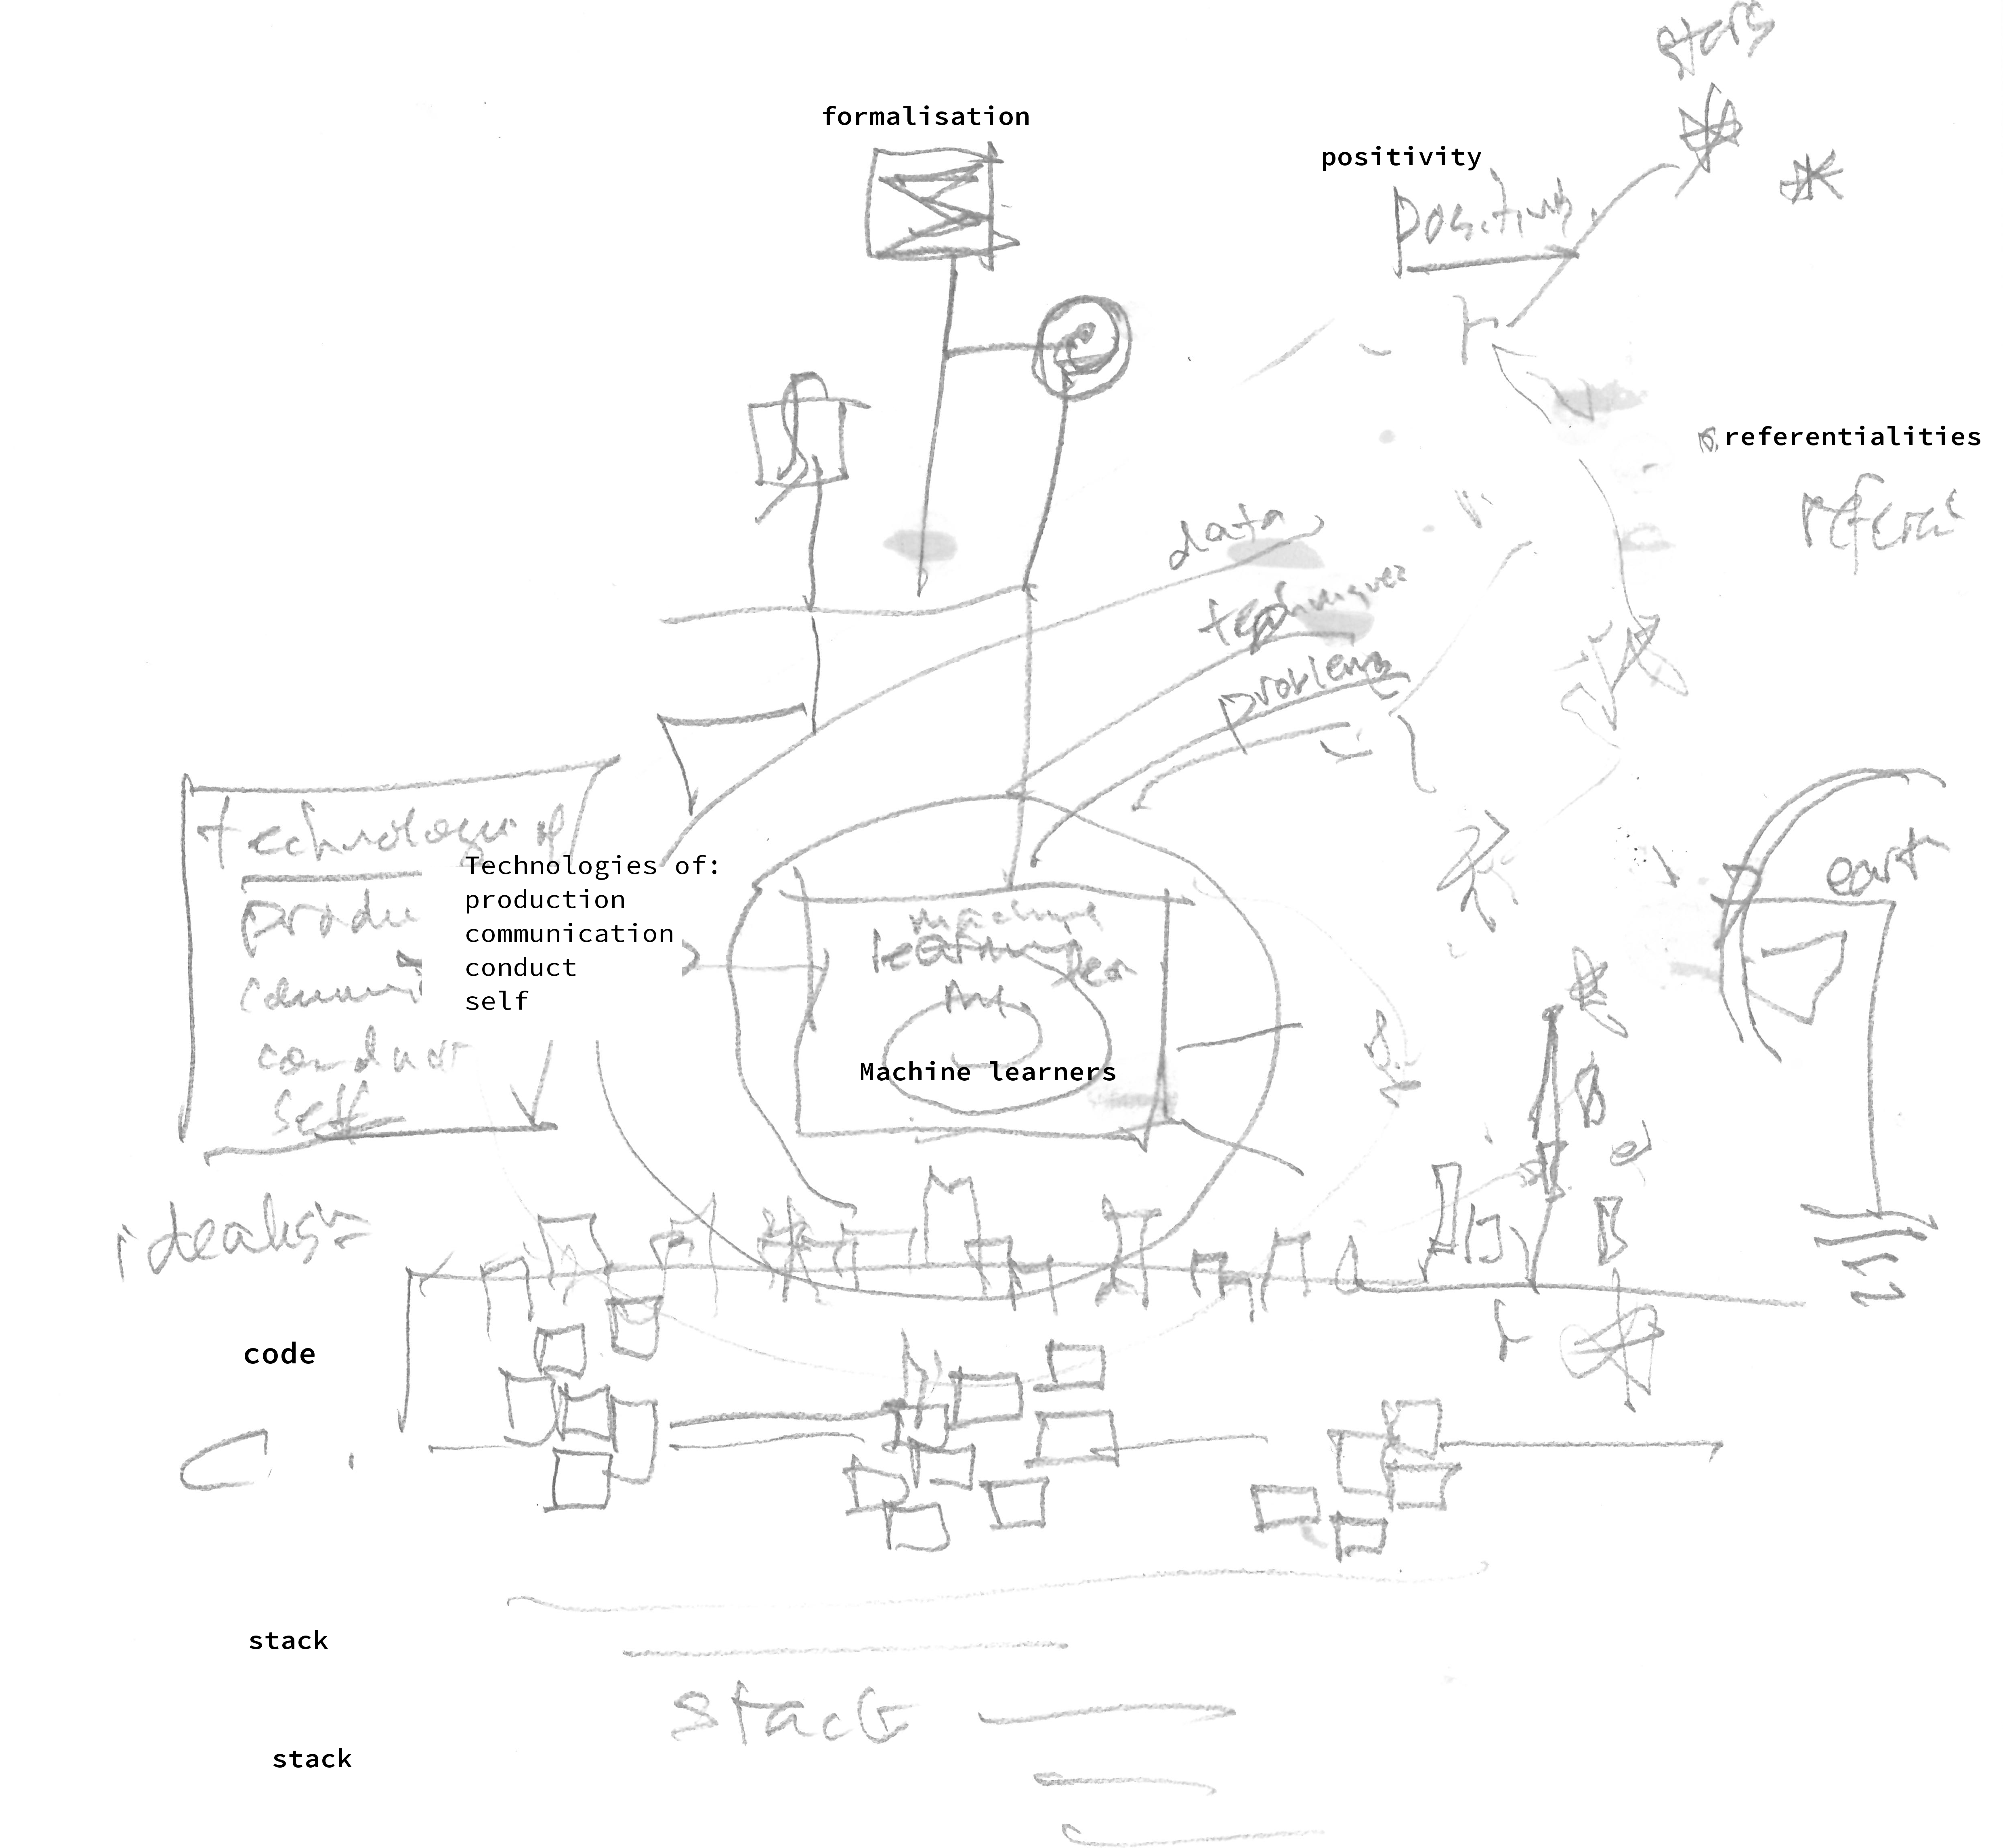
\includegraphics[width=0.9\textwidth]{figure/vast_diagram}
        \caption{Elements of learning to machine learn}
  \label{fig:vast_diagram}
\end{figure}

Some broadly shared topic structures help in any navigation of the
software libraries, pedagogical and research literatures. The textbooks,
the how-to recipe books
\autocites{Segaran_2007}{Kirk_2014}{Russell_2011}{Conway_2012} and the
online university courses on machine learning often have a similar topic
structure. \index{machine learning!topic structure of} They nearly
always begin with `linear models' (fitting a line to the data), then
move to logistic regression (a way of using the linear model to classify
binary outcomes; for example, spam/not-spam; malignant/benign;
cat/non-cat), and afterwards move to some selection of neural networks,
decision trees, support vector machine and clustering algorithms.
\index{linear regression} They add in some decision theory, techniques
of optimization, and ways of selecting predictive models (especially the
bias-variance trade-off).{[}\^{}1.62{]} The topic structures have in
recent years started to become increasingly uniform. This coagulation
around certain topics, problems and mathematical formalisms is both
something worth analyzing (since, for instance, it definitely affects
how machine learning is taken up in different settings), but should not
be taken as obvious or given since it results from many iterations.

Amidst this avalanching machine learning materials and practice, a
single highly cited and compendious textbook, \emph{Elements of
Statistical Learning: Data Mining, Inference, and Prediction} dating
from from around 2000 and currently in its second edition
\autocite{Hastie_2009}, can be seen from almost any point of the
terrain.\footnote{The complete text of the book can be downloaded from
  the website \url{http://statweb.stanford.edu/~tibs/ElemStatLearn/}. At
  the end of short intensive course on data mining at the Centre of
  Postgraduate Statistics, Lancaster University, the course convenor,
  Brian Francis, recommended this book as the authoritative text. Some
  part of me rues that day. That book is a poisoned chalice; that is,
  something shiny, valuable but also somewhat toxic.}
\index{Elements of Statistical Learning@\textit{Elements of Statistical Learning}}
At least for archaeological purposes, I regard this book as an
assemblage, \index{archaeology!assemblages in} and a diagram that
presents many important statements, forms of visibility and relations
between forces at work in machine learning. The authors of the book,
Jeff Hastie, Rob Tibshirani and Jerome Friedman \index{Hastie, Jeff}
\index{Tibshirani, Rob} \index{Friedman, Jerome} are statisticians
working at Stanford and Columbia University.

\emph{Elements of Statistical Learning} is a massive textual object,
densely radiant with equations, tables, algorithms, graphs and
references to other scientific literature. From the first pages proper
of the book, almost every page has a figure or a table or a formal
algorithm (counting these together: 1670 equations; 291 figures; 34
tables; and 94 algorithms, giving a total of 2089 operational statements
threaded through the book). Equations rivet the text with mathematical
abstractions of varying sophistication. On each page of the book we are
seeing, reading, puzzling over and perhaps learning from the products of
code execution. The graphic figures are all produced by code. The tables
are mostly produced by code. The algorithms specify how to implement
code, and the equations diagram various operations, spaces and movements
that meant to run as code.

In the range of references, combinations of code, diagram, equation,
scientific disciplines and computational elements, and perhaps in the
somewhat viscous, inter-objectively diverse referentiality that impinges
on any reading of it, \emph{Elements of Statistical Learning} betrays
some hyperobject-like positivity \index{positivity}
\autocite{Morton_2013}. \index{hyperobject} It is an accumulation of
forms, techniques, practices, propositions and referential relations.
\emph{Elements of Statistical Learning} combines statistical science
with various algorithms to `learn from data' \autocite[1]{Hastie_2009}.
The data range across various kinds of problems (identifying spam email,
predicting risk of heart disease, recognising handwritten digits, etc.).
The learning takes the form of various machine learning techniques,
methods and algorithms (linear regression, k-nearest neighbours, neural
networks, support vector machines, the Google Page Rank algorithm,
etc.).

There are other juggernaut machine learning textbooks.
\index{machine learning!textbooks} Ethem Alpaydin's \emph{Introduction
to Machine Learning} \autocite{Alpaydin_2010} (a more computer
science-base account), Christopher Bishop's heavily mathematical
\emph{Pattern recognition and machine learning} \autocite{Bishop_2006},
Brian Ripley's luminously illustrated and almost coffee-table formatted
\emph{Pattern Recognition and Neural Networks} \autocite{Ripley_1996}
\index{Ripley, Brian}, Tom Mitchell's earlier artificial
intelligence-centred \emph{Machine learning} \autocite{Mitchell_1997}
\index{Mitchell, Tom}, Peter Flach's perspicuous \emph{Machine Learning:
The Art and Science of Algorithms that Make Sense of Data}
\autocite{Flach_2012} \index{Flach, Peter}, or further afield, the
sobering and laconic \emph{Statistical Learning for Biomedical Data}
\autocite{Malley_2011} all cover a similar range of data and approaches.
These and quite a few other recent machine learning textbooks display a
range of emphases, ranging from the highly theoretical to the very
practical, from an orientation to statistical inference to an emphasis
on computational processes, from science to commercial applications.

\section{Who reads machine learning
textbooks?}\label{who-reads-machine-learning-textbooks}

How does such textbook help us assess and engage with claim to learn
from data or to produce knowledge differently? While it certainly does
not comprehend everything taking place in and around machine learning,
it diagrams several \emph{elementary} tendencies or traits.
\index{\textit{Elements of Statistical Learning}!as diagram of abstraction}
It's readership as we will see is widespread. It has a heterogeneous
texture in terms of the examples, formalisms, disciplines and domains it
covers. It starkly renders the problems of making sense of mathematical
operations, diagrams and transformations carried on through calculation,
simulation, deduction or analysis. It draws on a matrix of operational
practices, particularly in the form of the \texttt{R} code it heavily
but somewhat latently relies on. In short, \emph{Elements of Statistical
Learning} presents a multi-faceted and somewhat monumental layering of
abstractive practice that might be open to archaeological inquiry.

\begin{table}[ht]
\centering
\begingroup\tiny
\begin{tabular}{p{0.1\textwidth}p{0.85\textwidth}}
  \hline
Citations & Field \\ 
  \hline
556 & Engineering \\ 
  520 & Computer Science \\ 
  380 & Engineering", "Computer Science \\ 
  369 & Biotechnology \& Applied Microbiology \\ 
  344 & Mathematical \& Computational Biology \\ 
  207 & Mathematics", "Computer Science \\ 
  175 & Chemistry \\ 
  150 & Remote Sensing \\ 
  116 & Instruments \& Instrumentation \\ 
   99 & Imaging Science \& Photographic Technology", "Computer Science \\ 
   81 & Engineering", "Automation \& Control Systems \\ 
   77 & Mathematics", "Biochemistry \& Molecular Biology \\ 
   77 & Public, Environmental \& Occupational Health \\ 
   75 & Medical Informatics \\ 
   69 & Mathematics \\ 
   69 & Operations Research \& Management Science", "Computer Science \\ 
   67 & Research \& Experimental Medicine \\ 
   66 & Geology \\ 
   62 & Marine \& Freshwater Biology \\ 
   60 & Engineering", "Engineering \\ 
   \hline
\end{tabular}
\endgroup
\caption{Subject categories of research publications citing \textit{Elements of Statistical Learning} 2001-2015. The subject categories derive from Thomson-Reuter \textit{Web of Science}.} 
\label{tab:fields_citing_hastie}
\end{table}

Who reads the \emph{Elements of Statistical Learning}?
\index{\textit{Elements of Statistical Learning}!readerships} It is
often cited by academic machine learning practitioners as an
authoritative guide. On the other hand, students participating in new
data science courses often come from different disciplinary backgrounds
and find the tome unhelpful (see the comment by students during an
introductory data science course documented in \autocite{Schutt_2013}).
Whether the citations are friendly or not, it is hard to find a field of
contemporary science, engineering, natural, applied, health and indeed
social science that has not cited it. A Thomson-Reuters Scientific `Web
of Science'(TM) search for references citing either the first or second
edition of \autocite{Hastie_2009} yields around 9000 results. These
publications sprawl across over 100 different fields of research.
\index{science!diversity of fields in machine learning} While computer
science, mathematics and statistics dominate, a very diverse set of
references comes from disciplines from archaeology, through fisheries
and forestry, genetics, robotics, telecommunications and toxicology
ripple out from this book since 2001. Table
\ref{tab:fields_citing_hastie} shows the top 20 fields by count. One
could learn something about the diagrammatic movement of machine
learners from that reference list, which itself spans biomedical,
engineering, telecommunications, ecology, operations research and many
other fields. While it is not surprising to see computer science,
mathematics and engineering appearing at highest concentration in the
literature, molecular biology, control and automation, operation
research, business and public health soon appear, suggesting something
of the propagating accumulation or positivity of machine learning.
\index{positivity!as form of accumulation}

\begin{figure}
  \centering
      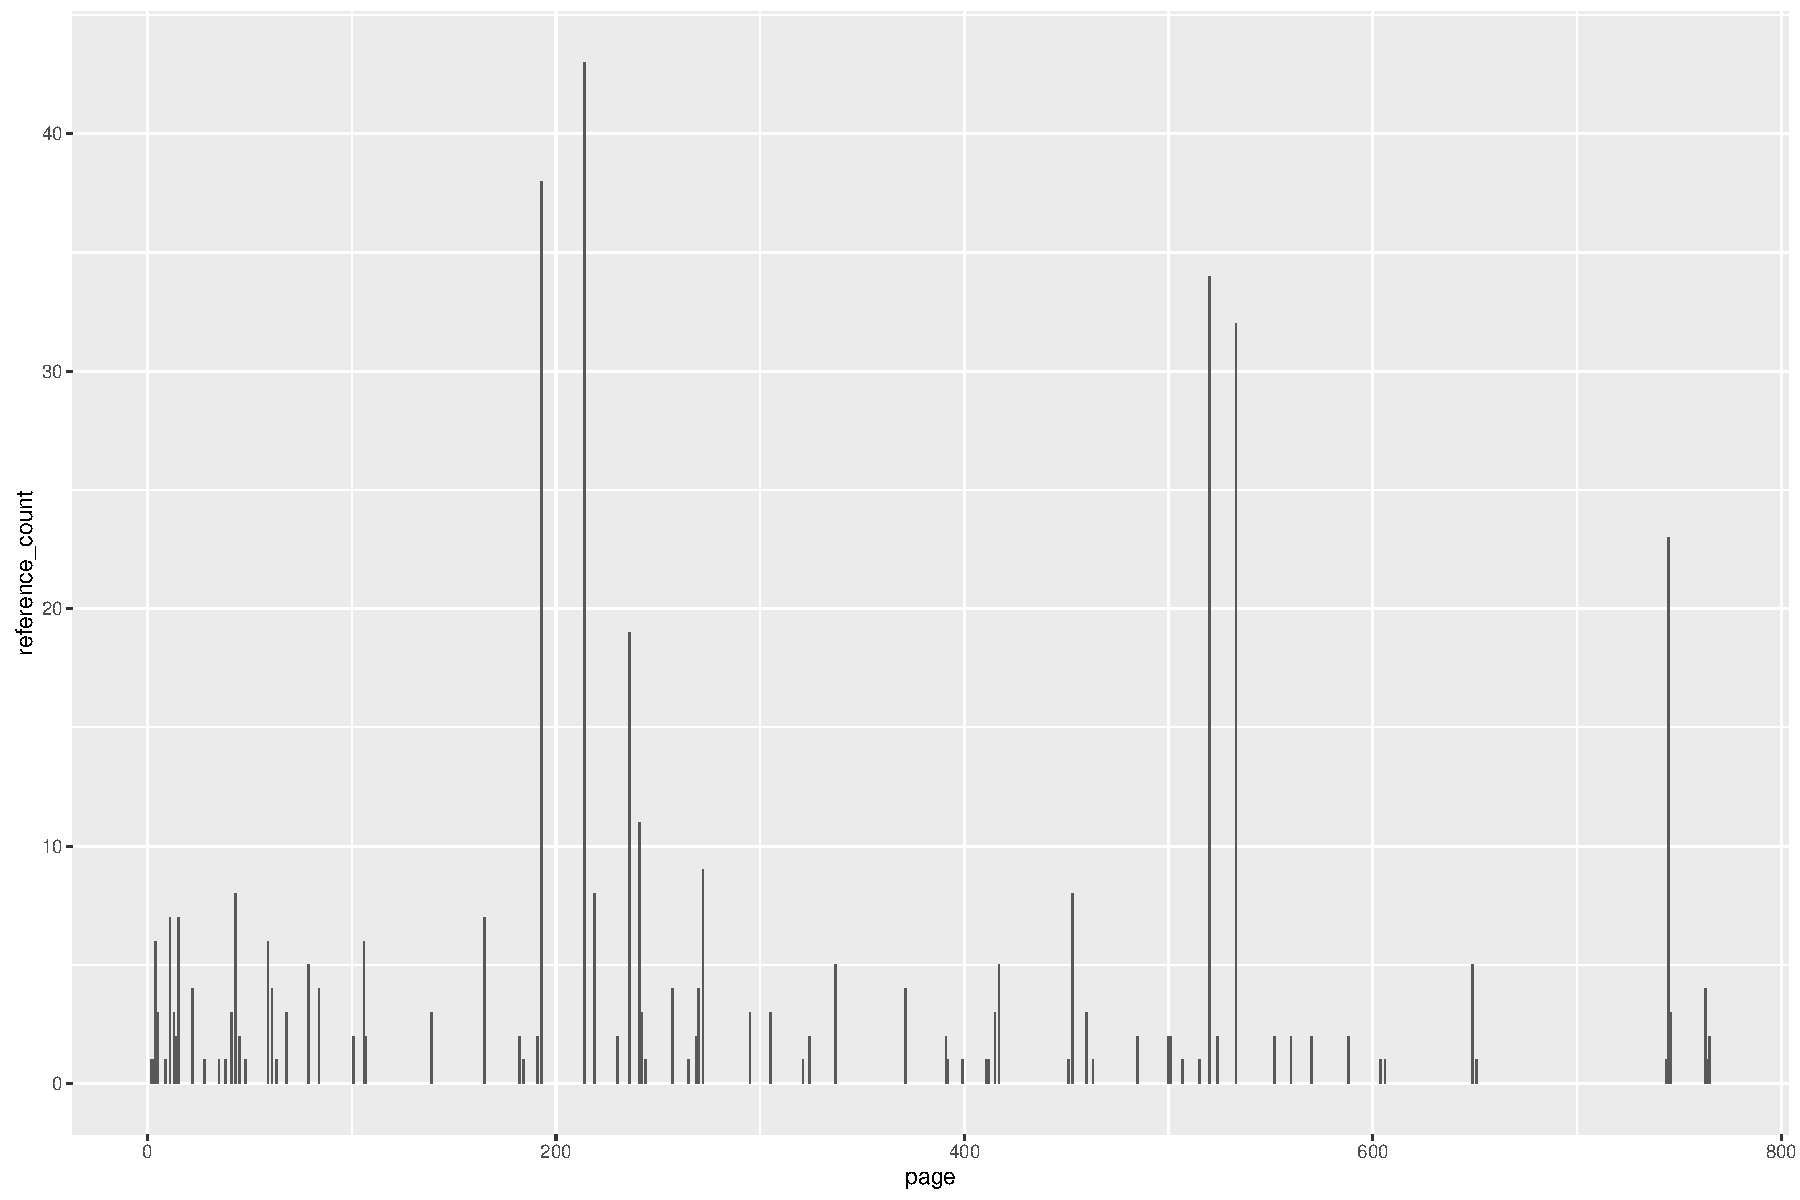
\includegraphics[width=0.9\textwidth]{figure/plot_hastie_pages-1.pdf}
        \caption[Pages cited from \textit{Elements of Statistical Learning }]{Pages cited from \textit{Elements of Statistical Learning }  by academic publications in all fields.}
  \label{fig:hastie_pages}
\end{figure}

So we know that \emph{Elements of Statistical Learning} passes into many
fields. But what do people read in the textual environment of book? In
general, the thousands of citations of the book themselves compose a
diagram of the book's intersection with different domains of knowledge.
The relative concentrations and sparsities of these citations suggest
there may be specific sites of engagement in the techniques, approaches
and machines that the book documents. Of the around 760 pages in the two
editions (\autocite{Hastie_2009} and \autocite{Hastie_2001}), around 83
distinct pages are referenced in the citing literature. As figure
\ref{fig:hastie_pages} indicates, certain portions of the book are much
more heavily cited than others. This distribution of page references in
the literature that cites \emph{Elements of Statistical Learning} is a
rough guide to how the book has been read in different settings. For
instance, the most commonly cited page in the book is page 553. That
page begins a section called `Non-negative Matrix Factorization',
\index{machine learner!Non-negative matrix factorization} a technique
frequently used to process digital images to compress their visual
complexity into a simpler set of visual signals
\autocite[553]{Hastie_2009}. (The underlying reference here is the
highly cited paper \autocite{Lee_1999}) Like \texttt{kittydar}, it, as
Hastie and co-authors write, `learns to represent faces with a set of
basis images resembling parts of faces' \autocite[555]{Hastie_2009}. (So
\texttt{kittydar}, which doesn't use NMF, might do better if it did,
because it could work just with parts of the images that lie somewhere
near the parts of a cat's face -- its nose, its eyes, its
ears.\index{machine learner!\texttt{kittydar}}) \index{face recognition}

Conversely, what do the authors of \emph{Elements of Statistical
Learning} read? The book gathers elements from many different quarters
and seeks to integrate them in terms of statistical theory. The
hyperobject-like aspect of the book comes from the thick weave of
equations, diagrams, tables, algorithms, bibliographic apparatus, and
numbers wreathed in typographic ornaments drawn from many other sources.
For instance, in terms of outgoing references or the literature that it
cites, \emph{Elements of Statistical Learning} webs together a field of
scientific and technical work with data and predictive models ranging
across half a century. The reference list beginning at page 699
\autocite[699]{Hastie_2009} runs for around 35 pages, and the five
hundred or so references there point in many directions. The weave of
these elements differs greatly from citational patterns in the
humanities or social sciences. Reading this book almost necessitates an
archaeological approach since it comprises so many parts and fragments.
\index{archaeology!reading practices in}

\begin{figure}
  \centering
      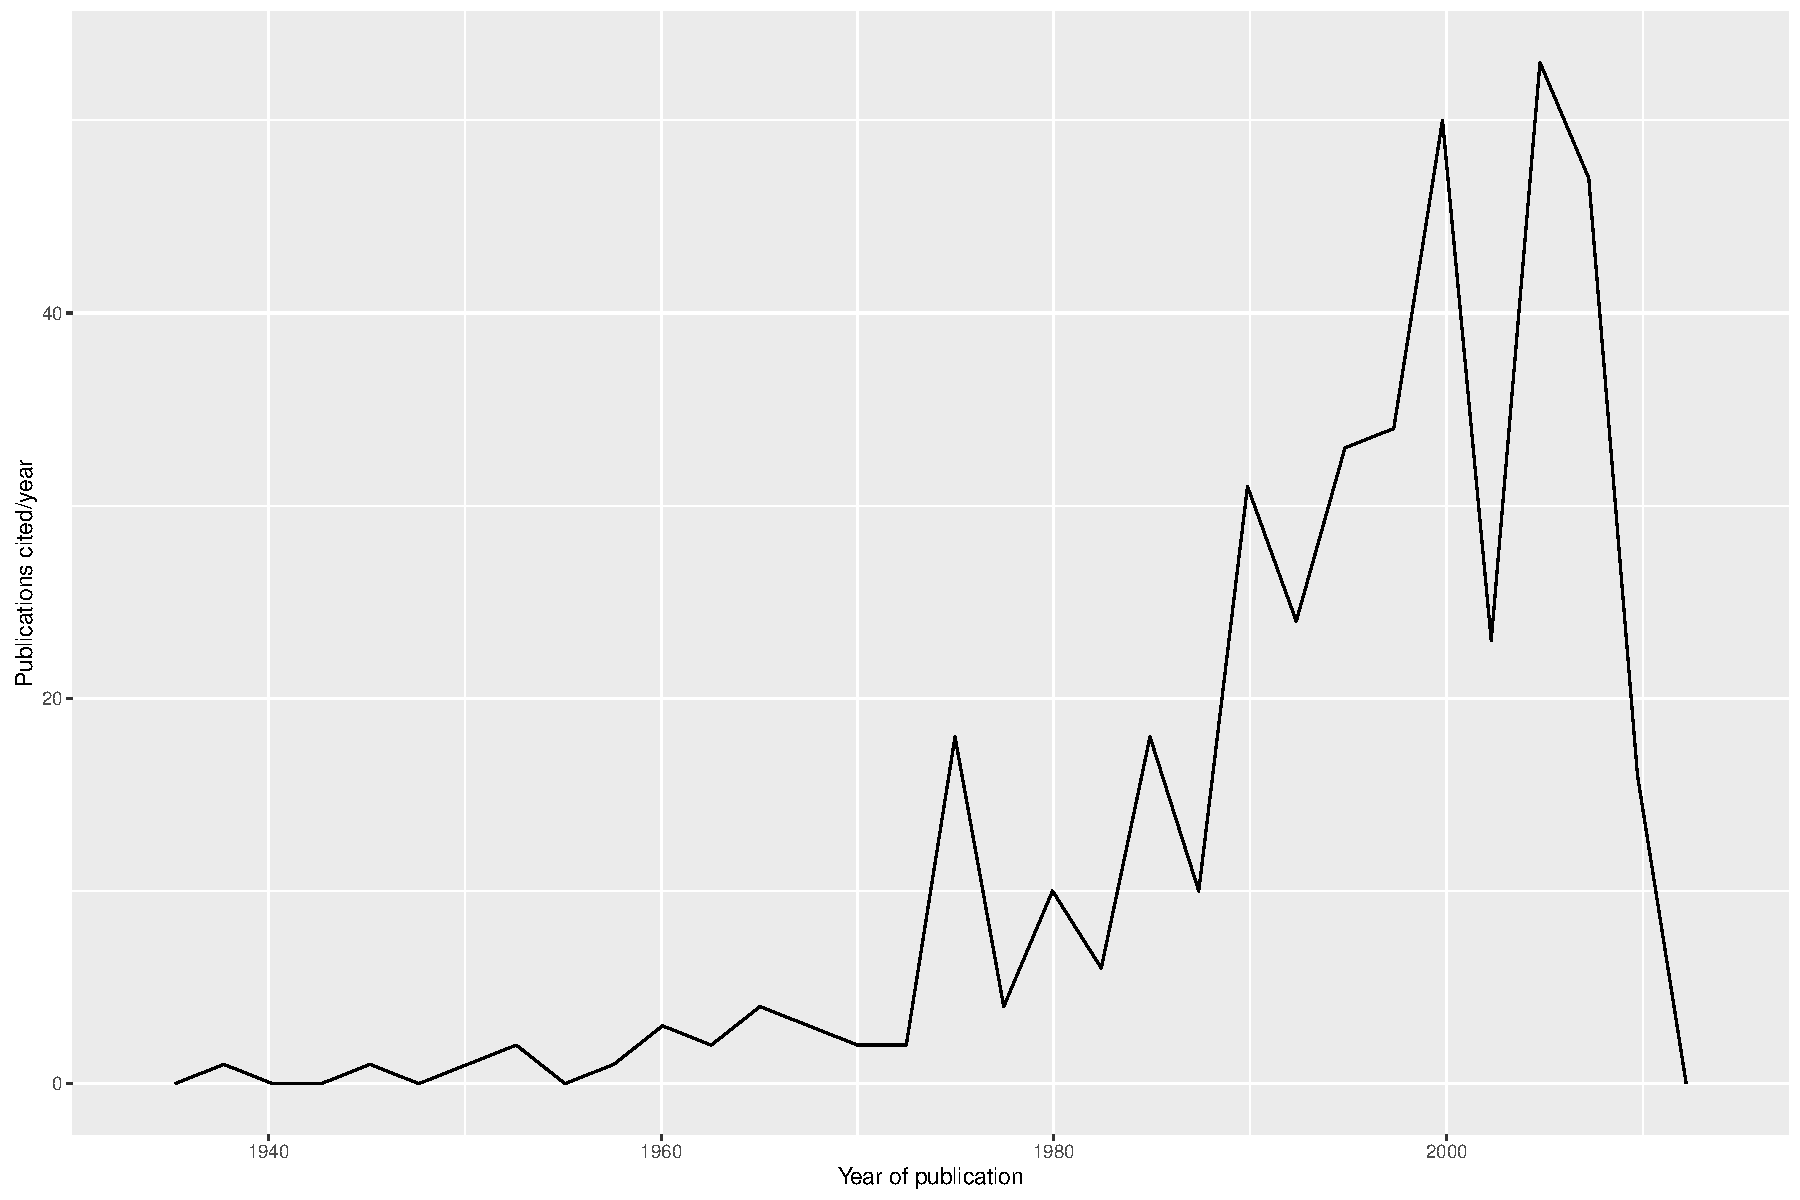
\includegraphics[width=0.9\textwidth]{figure/hastie_references-1.pdf}
        \caption[Publications cited in \textit{Elements of Statistical Learning}]{Publications cited in\textit{Elements of Statistical Learning}. The references range over almost 80 years, with peaks in late 1970s, late 1980s, mid-1990s and mid-2000s. These peaks relate to different mixtures of cybernetics, statistics, computer science, medicine, biology and other fields running through machine learning. Regression-related publications form the main body of citation. }
  \label{fig:hastie_cited_refs}
\end{figure}

The citational fabric of \emph{Elements of Statistical Learning} is
woven with different threads, some reaching back into early twentieth
statistics, some from post-WW2 cybernetics, many from information theory
and then in the 1980s onwards, increasingly, from cognitive science and
computer science (see figure \ref{fig:hastie_cited_refs} to get some
sense of their distribution over time). While some of these references
either point to Hastie, Tibshirani or Friedman's own publications, or
that of their statistical colleagues, the references rove quite widely
in other fields and over time. \emph{Elements of Statistical Learning}
as a text is processing, assimilating and recombining techniques,
diagrams and data from many different places and times. (The different
waves appearing in the references cited in \autocite{Hastie_2009} will
shape discussion in later chapters in certain ways; for instance, late
1990s biology is the topic of chapter \ref{ch:genome} and optimization
functions dating from the 1950s are discussed in chapter
\ref{ch:function}).

Both the inward and outward movements of citation suggest that
\emph{Elements of Statistical Learning}, like much in field of machine
learning, has a matrix-like character that constantly superimposes and
transposes elements across boundaries and barriers. The implication here
is that machine learning as a knowledge practice has a highly interwoven
texture, and in this respect differs somewhat from the classical
understandings of scientific disciplines as bounded by communities of
practice, norms and problems (as for instance, in Thomas Kuhn's account
of normal science \autocite{Kuhn_1996}. \index{Kuhn, Thomas} This
aggregate or superimposed character of machine learning should
definitely figure in any sense we make of it, and will inevitably affect
how critical thought might test itself against it.
\index{critical thought}.

\section{\texorpdfstring{\texttt{R}: a matrix of
transformations}{R: a matrix of transformations}}\label{r-a-matrix-of-transformations}

\index{programming languages!R|(} Although barely a single line of code
appears in \emph{Elements of Statistical Learning}, all of the learners
presented there are implemented in a single programming language,
\texttt{R}. Coding is the operational practice that links the different
planes and elements of machine learning in an operational formation.
\index{operational formation!code as operational practice in}
\index{code!as operational practice} The authors say `we used the R and
S-PLUS programming languages in our courses' \autocite[9]{Hastie_2009}
but many elements of the book derive from \texttt{R} code.{[}\^{}1.91{]}
The proliferation of programming languages such as \texttt{FORTRAN}
(dating from the 1950s), \texttt{C} (1970s), \texttt{C++} (1980s), then
\texttt{Perl} (1990s), \texttt{Java} (1990s), \texttt{Python} (1990s)
and \texttt{R} (1990s), and computational scripting environments such as
Matlab, multiplied the paths along which machine learners move through
operational formations.\index{programming languages} It would be
difficult to comprehend the propagation of machine learners across
domains of science, business and government without paying attention to
coding practices. Even if textbooks and research articles are not read,
software packages and libraries for machine learning are used. Code has
a mobility that extends the diagrammatic practices of machine learning
into a variety of settings and places where the scientific reading
apparatuses of equations, statistical plots, and citations of research
articles would not be operative. \index{code!mobility of}

\begin{verbatim}
## Error in install.packages(new.packages, dependencies = "Suggests", repos = "http://cran.us.r-project.org"): unable to install packages
\end{verbatim}

\begin{verbatim}
## Error in contrib.url(getOption("repos"), type): trying to use CRAN without setting a mirror
\end{verbatim}

\begin{verbatim}
## Error in as.data.frame(pack): object 'pack' not found
\end{verbatim}

\begin{verbatim}
## Error in table(pack_df["Suggests"]): object 'pack_df' not found
\end{verbatim}

\begin{verbatim}
## Error in `colnames<-`(`*tmp*`, value = "How often suggested"): attempt to set 'colnames' on an object with less than two dimensions
\end{verbatim}

\begin{verbatim}
## Error in UseMethod("xtable"): no applicable method for 'xtable' applied to an object of class "function"
\end{verbatim}

\begin{verbatim}
## Error in table(pack_df["Depends"]): object 'pack_df' not found
\end{verbatim}

\begin{verbatim}
## Error in rownames(df2): object 'df2' not found
\end{verbatim}

\begin{verbatim}
## Error in colnames(df2) = c("Package", "How often depended on"): object 'df2' not found
\end{verbatim}

\begin{verbatim}
## Error in eval(expr, envir, enclos): object 'df2' not found
\end{verbatim}

\begin{verbatim}
## Error in xtable(df3[1:20, ], caption = c("`R` packages depended on by the `ElemStatLearn` package", : object 'df3' not found
\end{verbatim}

\begin{verbatim}
## Error in print(table1, type = "latex", table.placement = "!htb"): object 'table1' not found
\end{verbatim}

\begin{verbatim}
## Error in print(table2, type = "latex", table.placement = "!htb"): object 'table2' not found
\end{verbatim}
